\documentclass[aspectratio=169,12pt,xcolor=table]{beamer}

% Modern theme
\usetheme{Madrid}
\usecolortheme{whale}

% Packages
\usepackage[utf8]{inputenc}
\usepackage[T1]{fontenc}
\usepackage{amsmath}
\usepackage{amsfonts}
\usepackage{amssymb}
\usepackage{graphicx}
\usepackage{booktabs}
\usepackage{tikz}
\usepackage{pgfplots}
\pgfplotsset{compat=1.18}
\usepackage{multicol}
\usepackage{adjustbox}
\usepackage{hyperref}

% Custom colors
\definecolor{niftyblue}{RGB}{0,71,171}
\definecolor{niftyorange}{RGB}{255,140,0}
\definecolor{niftygreen}{RGB}{34,139,34}
\definecolor{niftyred}{RGB}{220,20,60}
\definecolor{lightgray}{RGB}{240,240,240}

% Theme customization
\setbeamercolor{palette primary}{bg=niftyblue,fg=white}
\setbeamercolor{palette secondary}{bg=niftyorange,fg=white}
\setbeamercolor{palette tertiary}{bg=niftygreen,fg=white}
\setbeamercolor{palette quaternary}{bg=niftyblue,fg=white}
\setbeamercolor{structure}{fg=niftyblue}
\setbeamercolor{section in toc}{fg=niftyblue}
\setbeamercolor{subsection in toc}{fg=niftyorange}
\setbeamercolor{frametitle}{bg=niftyblue,fg=white}
\setbeamercolor{block title}{bg=niftyblue,fg=white}
\setbeamercolor{block body}{bg=lightgray,fg=black}

% Custom footer with full blue background
\setbeamertemplate{footline}{
  \leavevmode%
  \hbox{%
  \begin{beamercolorbox}[wd=.5\paperwidth,ht=2.5ex,dp=1ex,center,sep=0pt]{palette quaternary}%
    \usebeamerfont{title in head/foot}\insertshorttitle
  \end{beamercolorbox}%
  \begin{beamercolorbox}[wd=.5\paperwidth,ht=2.5ex,dp=1ex,right,sep=0pt]{palette quaternary}%
    \usebeamerfont{date in head/foot}\insertshortdate{}\hspace*{2em}
    \insertframenumber{} / \inserttotalframenumber\hspace*{2ex} 
  \end{beamercolorbox}}%
  \vskip0pt%
}

% Remove navigation symbols
\setbeamertemplate{navigation symbols}{}

% Hyperref setup
\hypersetup{
    colorlinks=true,
    linkcolor=niftyblue,
    urlcolor=niftyblue,
    citecolor=niftyblue
}

% Title information
\title[Short Title]{Presentation Title}
\subtitle{Presentation Subtitle}
\author[Author Names]{Author Name(s)}
\institute[Institution]{
    Department Name \\
    Institution Name
}
\date{\today}

\begin{document}

% ========================= SLIDE 1: TITLE =========================
\begin{frame}[plain]
\vspace{0.5cm}
\titlepage
\vspace{-1.2cm}
\begin{center}
    \textcolor{niftyorange}{\rule{0.8\textwidth}{2pt}}
    \vspace{0.1cm}
    
    {\small \textit{Course Name}} \\
    \vspace{0.1cm}
    {\small \textit{Academic Information}} \\
    \vspace{0.2cm}
    {\small \today}
\end{center}
\end{frame}

% ========================= SLIDE 2: OUTLINE =========================
\begin{frame}[allowframebreaks]{Presentation Outline}
\tableofcontents[hideallsubsections]
\end{frame}

% ========================= SECTION 1: INTRODUCTION =========================
\section{Introduction}

\begin{frame}{Introduction}
\begin{columns}[T]
\begin{column}{0.5\textwidth}
    \textbf{Key Points:}
    \begin{itemize}
        \item First point
        \item Second point
        \item Third point
    \end{itemize}
    
    \vspace{0.5cm}
    \textbf{Background:}
    \begin{itemize}
        \item Context information
        \item Relevant details
        \item Important notes
    \end{itemize}
\end{column}

\begin{column}{0.5\textwidth}
    \begin{block}{Research Focus}
        \textcolor{niftyblue}{\textbf{Main hypothesis or research question goes here}}
    \end{block}
    
    \vspace{0.3cm}
    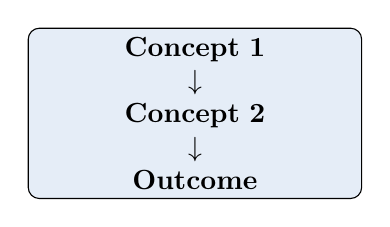
\begin{tikzpicture}
        \node[draw, fill=niftyblue!10, rounded corners, text width=4cm, align=center] at (0,0) {
            \textbf{Concept 1} \\
            $\downarrow$ \\
            \textbf{Concept 2} \\
            $\downarrow$ \\
            \textbf{Outcome}
        };
    \end{tikzpicture}
\end{column}
\end{columns}
\end{frame}

% ========================= SECTION 2: METHODOLOGY =========================
\section{Methodology}

\begin{frame}{Mathematical Formulation}
\begin{columns}[T]
\begin{column}{0.55\textwidth}
    \textbf{Main Formula:}
    \begin{equation*}
        \boxed{f(x) = ax^2 + bx + c}
    \end{equation*}
    
    \vspace{0.1cm}
    \textbf{Where:}
    \begin{itemize}
        \item $f(x)$ = Function value
        \item $a, b, c$ = Parameters
        \item $x$ = Variable
    \end{itemize}
    
    \vspace{0.2cm}
    \textbf{Interpretation:}
    \begin{itemize}
        \item Explanation point 1
        \item Explanation point 2
        \item Explanation point 3
    \end{itemize}
\end{column}

\begin{column}{0.45\textwidth}
    \begin{block}{Example}
        Sample calculation or example goes here
    \end{block}
    
    \vspace{0.2cm}
    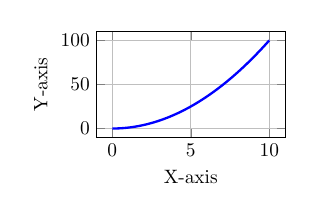
\begin{tikzpicture}[scale=0.7]
        \begin{axis}[
            xlabel={X-axis},
            ylabel={Y-axis},
            domain=0:10,
            samples=100,
            grid=major,
            width=5cm,
            height=3.5cm
        ]
        \addplot[blue, very thick] {x^2};
        \end{axis}
    \end{tikzpicture}
\end{column}
\end{columns}
\end{frame}

\begin{frame}{Data \& Analysis}
\begin{columns}[T]
\begin{column}{0.5\textwidth}
    \textbf{Data Sources:}
    \begin{itemize}
        \item Source 1
        \item Source 2
        \item Source 3
    \end{itemize}
    
    \vspace{0.3cm}
    \textbf{Analysis Steps:}
    \begin{enumerate}
        \item Step 1: Description
        \item Step 2: Description
        \item Step 3: Description
        \item Step 4: Description
    \end{enumerate}
\end{column}

\begin{column}{0.5\textwidth}
    \begin{table}[h]
    \small
    \begin{tabular}{lcc}
    \toprule
    \textbf{Item} & \textbf{Value 1} & \textbf{Value 2} \\
    \midrule
    \rowcolor{niftyblue!20} Item A & 10.5 & 12.3 \\
    Item B & 8.7 & 9.2 \\
    \rowcolor{lightgray} Item C & 15.2 & 14.8 \\
    Item D & 11.3 & 10.9 \\
    \bottomrule
    \end{tabular}
    \end{table}
    
    \vspace{0.2cm}
    \begin{block}{Note}
        Additional context or explanation
    \end{block}
\end{column}
\end{columns}
\end{frame}

% ========================= SECTION 3: RESULTS =========================
\section{Results}

\begin{frame}{Key Findings}
\begin{center}
\textbf{\Large Main Result Statement}
\end{center}

\vspace{0.1cm}
\begin{table}[h]
\centering
\small
\begin{tabular}{clcc}
\toprule
\textbf{Rank} & \textbf{Category} & \textbf{Metric 1} & \textbf{Metric 2} \\
\midrule
1 & Category A & 95.3 & 88.2 \\
2 & Category B & 92.1 & 85.7 \\
\rowcolor{niftyblue!30} \textbf{3} & \textbf{Category C} & \textbf{90.8} & \textbf{84.3} \\
4 & Category D & 87.5 & 82.1 \\
5 & Category E & 85.2 & 79.8 \\
\bottomrule
\end{tabular}
\end{table}

\begin{block}{Key Insight}
\textcolor{niftyblue}{\textbf{Main takeaway from the results}}
\end{block}
\end{frame}

\begin{frame}{Visual Analysis}
\vspace{0.2cm}
\begin{columns}[c]
\begin{column}{0.5\textwidth}
    \centering
    % \includegraphics[width=\textwidth]{figure1.png}
    [Figure 1 Placeholder]
    \vspace{0.1cm}
    
    {\small \textbf{Figure 1 Caption}}
\end{column}
\begin{column}{0.5\textwidth}
    \centering
    % \includegraphics[width=\textwidth]{figure2.png}
    [Figure 2 Placeholder]
    
    {\small \textbf{Figure 2 Caption}}
\end{column}
\end{columns}
\end{frame}

\begin{frame}{Detailed Analysis}
\begin{columns}[T]
\begin{column}{0.5\textwidth}
    \textbf{Observation 1:}
    \begin{itemize}
        \item Detail A
        \item Detail B
        \item Detail C
    \end{itemize}
    
    \vspace{0.3cm}
    \textbf{Observation 2:}
    \begin{itemize}
        \item Detail A
        \item Detail B
        \item Detail C
    \end{itemize}
\end{column}

\begin{column}{0.5\textwidth}
    \begin{center}
    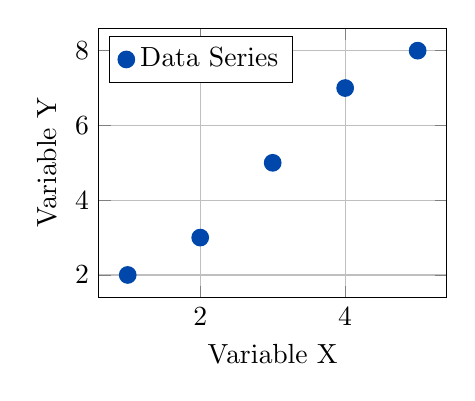
\begin{tikzpicture}
        \begin{axis}[
            xlabel={Variable X},
            ylabel={Variable Y},
            width=6cm,
            height=5cm,
            grid=major,
            legend pos=north west
        ]
        \addplot[only marks, mark=*, mark size=3pt, niftyblue] 
            coordinates {(1,2) (2,3) (3,5) (4,7) (5,8)};
        \addlegendentry{Data Series}
        \end{axis}
    \end{tikzpicture}
    \end{center}
\end{column}
\end{columns}
\end{frame}

% ========================= SECTION 4: DISCUSSION =========================
\section{Discussion}

\begin{frame}{Interpretation}
\begin{columns}[T]
\begin{column}{0.5\textwidth}
    \textbf{Main Points:}
    \begin{enumerate}
        \item \textcolor{niftygreen}{\textbf{Point 1}} \\
        Explanation and context
        
        \vspace{0.3cm}
        \item \textcolor{niftyblue}{\textbf{Point 2}} \\
        Explanation and context
        
        \vspace{0.3cm}
        \item \textcolor{niftyorange}{\textbf{Point 3}} \\
        Explanation and context
    \end{enumerate}
\end{column}

\begin{column}{0.5\textwidth}
    \begin{alertblock}{Important Note}
        \small
        Key conclusion or important observation
    \end{alertblock}
    
    \vspace{0.3cm}
    \begin{block}{Implication}
        Broader significance of findings
    \end{block}
\end{column}
\end{columns}
\end{frame}

\begin{frame}{Practical Applications}
\begin{center}
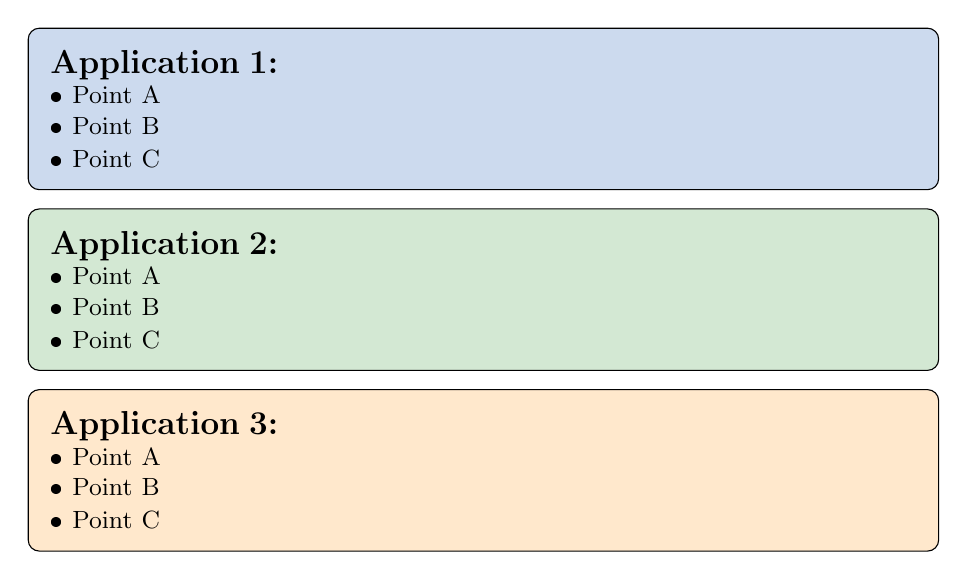
\begin{tikzpicture}[scale=0.85]
    \node[draw, fill=niftyblue!20, rounded corners, text width=11cm, align=left, inner sep=8pt] at (0,5.5) {
        \textbf{\large Application 1:} \\
        \small
        • Point A \\
        • Point B \\
        • Point C
    };
    
    \node[draw, fill=niftygreen!20, rounded corners, text width=11cm, align=left, inner sep=8pt] at (0,2.8) {
        \textbf{\large Application 2:} \\
        \small
        • Point A \\
        • Point B \\
        • Point C
    };
    
    \node[draw, fill=niftyorange!20, rounded corners, text width=11cm, align=left, inner sep=8pt] at (0,0.1) {
        \textbf{\large Application 3:} \\
        \small
        • Point A \\
        • Point B \\
        • Point C
    };
\end{tikzpicture}
\end{center}
\end{frame}

% ========================= SECTION 5: CONCLUSIONS =========================
\section{Conclusions}

\begin{frame}{Summary of Findings}
\begin{center}
\Large \textbf{Key Takeaways}
\end{center}

\vspace{0.1cm}
\begin{enumerate}
    \item \textcolor{niftyblue}{\textbf{Finding 1:}} \\
    Summary statement
    
    \vspace{0.1cm}
    \item \textcolor{niftygreen}{\textbf{Finding 2:}} \\
    Summary statement
    
    \vspace{0.1cm}
    \item \textcolor{niftyorange}{\textbf{Finding 3:}} \\
    Summary statement
    
    \vspace{0.1cm}
    \item \textcolor{niftyred}{\textbf{Finding 4:}} \\
    Summary statement
    
    \vspace{0.1cm}
    \item \textcolor{niftyblue}{\textbf{Finding 5:}} \\
    Summary statement
\end{enumerate}
\end{frame}

\begin{frame}{Limitations \& Future Work}
\begin{columns}[T]
\begin{column}{0.5\textwidth}
    \textbf{Limitations:}
    \begin{enumerate}
        \item Limitation 1
        \item Limitation 2
        \item Limitation 3
        \item Limitation 4
        \item Limitation 5
    \end{enumerate}
\end{column}

\begin{column}{0.5\textwidth}
    \textbf{Future Research:}
    \begin{enumerate}
        \item \textcolor{niftyblue}{\textbf{Direction 1}} \\
        Brief description
        
        \item \textcolor{niftygreen}{\textbf{Direction 2}} \\
        Brief description
        
        \item \textcolor{niftyorange}{\textbf{Direction 3}} \\
        Brief description
        
        \item \textcolor{niftyred}{\textbf{Direction 4}} \\
        Brief description
    \end{enumerate}
\end{column}
\end{columns}
\end{frame}

% ========================= CLOSING SLIDES =========================
\begin{frame}{References}
\small
\begin{enumerate}
    \item Author(s), ``Title,'' \textit{Journal/Conference}, Year. \\
    \textcolor{niftyblue}{\url{https://doi.org/...}}
    
    \vspace{0.2cm}
    \item Author(s), ``Title,'' \textit{Journal/Conference}, Year. \\
    \textcolor{niftyblue}{\url{https://doi.org/...}}
    
    \vspace{0.2cm}
    \item Author(s), ``Title,'' \textit{Journal/Conference}, Year. \\
    \textcolor{niftyblue}{\url{https://doi.org/...}}
\end{enumerate}
\end{frame}

\begin{frame}{Thank You!}
\begin{center}
{\Huge \textcolor{niftyblue}{\textbf{Questions?}}}

\vspace{1cm}
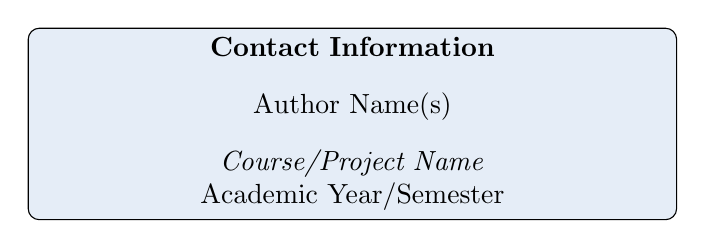
\begin{tikzpicture}
    \node[draw, fill=niftyblue!10, rounded corners, text width=8cm, align=center] {
        \textbf{Contact Information} \\
        \vspace{0.3cm}
        Author Name(s) \\
        \vspace{0.3cm}
        \textit{Course/Project Name} \\
        Academic Year/Semester
    };
\end{tikzpicture}

\vspace{0.2cm}
\textcolor{niftyorange}{\rule{0.6\textwidth}{2pt}}

\vspace{0.2cm}
\textit{\small "Memorable quote or tagline"}
\end{center}
\end{frame}

\end{document}
